\section{Pengantar Negative Feedback}

\subsection{Empat Jenis Negative Feedback}	
\begin{frame}{Empat Jenis Negative Feedback}	
	\begin{itemize}
		\item Negative feeback pertama $ \rightarrow $ menstabilkan voltage gain, meningkatkan impedansi input, menurunkan impedansi output
		\item Dengan adanya transistor \& op amps $\rightarrow$ bertambah 3 jenis negative feedback
	\end{itemize}
\end{frame}

\subsection{Ide Dasar}
\begin{frame}{Ide Dasar}
	\begin{itemize}
		\item Input dan output negative feedback amplifier bisa berupa tegangan maupun arus $ \rightarrow $ 4 tipe negative feedback
	\end{itemize}
	\begin{center}
		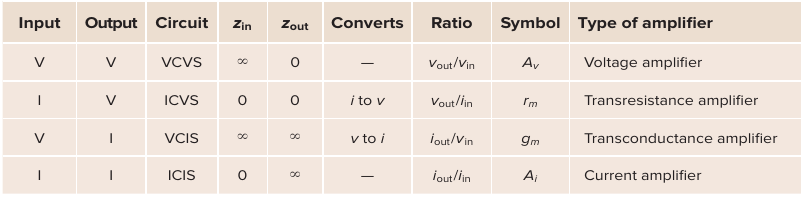
\includegraphics[width=\linewidth]{gambar/table-17.01}
	\end{center}
\end{frame}

\begin{frame}{Ide Dasar}
	\begin{itemize}
		\item \textbf{Jenis 1}: tegangan input dan tegangan output
		\begin{itemize}
			\item Rangkaian yang menggunakan negative feedback jenis ini disebut \textbf{voltage-controlled voltage source (VCVS)}
			\item Merupakan ideal voltage amplifier $ \rightarrow $ menstabilkan voltage gain, impedansi input tak hingga, impedansi output nol
		\end{itemize}
	
		\item \textbf{Jenis 2}: Arus input mengendalikan tegangan output
		\begin{itemize}
			\item Rangkaian yang menggunakan negative feedback jenis ini disebut \textbf{current-controlled voltage source (ICVS)}
			\item Disebut juga \textbf{transresistance amplifier} karena rasio dari $ v_{out}/i_{in} $ memliki satuan ohm
		\end{itemize}
	\end{itemize}
\end{frame}

\begin{frame}{Ide Dasar}
	\begin{itemize}	
		\item \textbf{Jenis 3}: Tegangan input mengendalikan arus output
		\begin{itemize}
			\item Rangkaian yang menggunakan negative feedback jenis ini disebut \textbf{voltage-controlled current source (VCIS)}
			\item Disebut juga \textbf{transconductance amplifier} karena rasio dari $ i_{out}/v_{in} $ memliki satuan mho
		\end{itemize}
		
		\item \textbf{Jenis 4:} Arus input dikuatkan untuk mendapatkan arus output yang lebih besar
		\begin{itemize}
			\item Rangkaian yang menggunakan negative feedback jenis ini disebut \textbf{current-controlled current source (ICIS)}
			\item Merupakan ideal current amplifier karena menstabilkan current gain, impedansi input nol dan impedansi ouput tak hingga
		\end{itemize}
	\end{itemize}
\end{frame}

\subsection{Konverter}
\begin{frame}{Konverter}
	\begin{itemize}
		\item Rangkaian VCVS dan ICIS disebut sebagai amplifier $ \rightarrow $ make sense, karena VCVS = voltage amplifier dan ICIS = current amplifier
		\item Namun bagaimana dengan transconductance dan transresistance amplifier ? $ \rightarrow $ input dan outputnya berbeda
		\item Rangkaian transconductance dan transresistance amplifier $ \rightarrow $ converter
		\item VCIS $\rightarrow$ voltage-to-current converter
		\item ICVS $\rightarrow$ current-to-voltage converter
	\end{itemize}
\end{frame}

\subsection{Diagram}
\begin{frame}{Diagram}
	\begin{figure}
		\centering
		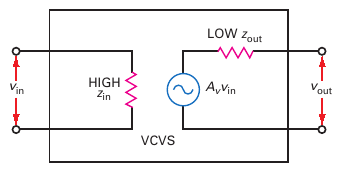
\includegraphics[width=0.7\linewidth]{gambar/fig-17.01a}
		\caption{Voltage-controlled voltage source}
		\label{fig-17.01a}
	\end{figure}
\end{frame}

\begin{frame}{Diagram}
	\begin{figure}
		\centering
		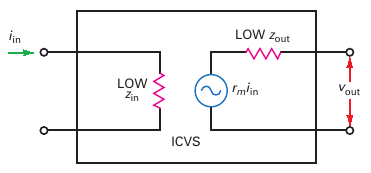
\includegraphics[width=0.7\linewidth]{gambar/fig-17.01b}
		\caption{Current-controlled voltage source}
		\label{fig-17.01b}
	\end{figure}
\end{frame}

\begin{frame}{Diagram}
	\begin{figure}
		\centering
		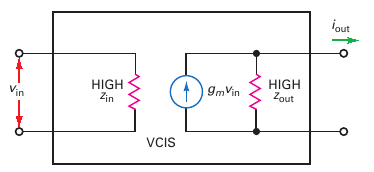
\includegraphics[width=0.7\linewidth]{gambar/fig-17.02a}
		\caption{Voltage-controlled current source}
		\label{fig-17.02a}
	\end{figure}
\end{frame}

\begin{frame}{Diagram}
	\begin{figure}
		\centering
		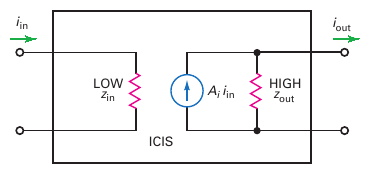
\includegraphics[width=0.7\linewidth]{gambar/fig-17.02b}
		\caption{Current-controlled current source}
		\label{fig-17.02b}
	\end{figure}
\end{frame}